\chapter{Results of the DAQ Tests}


\section{GANDALF Clock Frequency and ADC Test}
Before using the \ac{gandalf} modules in the \ac{daq}, they need to be checked for proper functioning.
For this, two things are relevant:
One is the quality of the sampling clock, the other the differential linearity and monotonyty of the \acp{adc}.
To perform these tests, a \SI{150}{\mega\hertz} sine voltage signal was generated with an AWG and a narrow bandwith \SI{150}{\mega\hertz} filter with a \SI{3}{\decibel} bandwidth of \SI{+-5}{\mega\hertz} \cite{}.
The filter ensures a pure sine wave and unwanted frequencies are suppressed.
The clean sine signal was then connected to the inputs of the \acp{gandalf}, one after another.
For each input \num{1000} waveforms were recorded, each with 430 samples.
For each channel a \ac{fft} was done for one waveform using the python3 functions \textit{scipy.fft.rfft} and \textit{scipy.fft.rfftfreq} to find the sampled frequencies in the signal.
\autoref{fig:gandalf_input_g23_ch0} shows the plot with the \ac{fft} for channel 0 of the \ac{amc} 46 used with the \ac{gandalf} 23.
In the plot the red line marks the center frequency of the measured signal.
%The measured values and the corresponding uncertainties are listed in \autoref{tab:gandalf_sin_150}.
The measured peak frequency is determined by the maxima in the frequency spectrum and the uncertainty is estimated to be halfe the frequency steps of the \ac{fft}.
The result of the \ac{fft} is a measured center frequency of \SI{149.4(10)}{\mega\hertz}.
Therefore the sampling frequency of the \ac{gandalf} is as intended, which means that the external clock signal is working correctly.
\begin{figure}
	\centering
	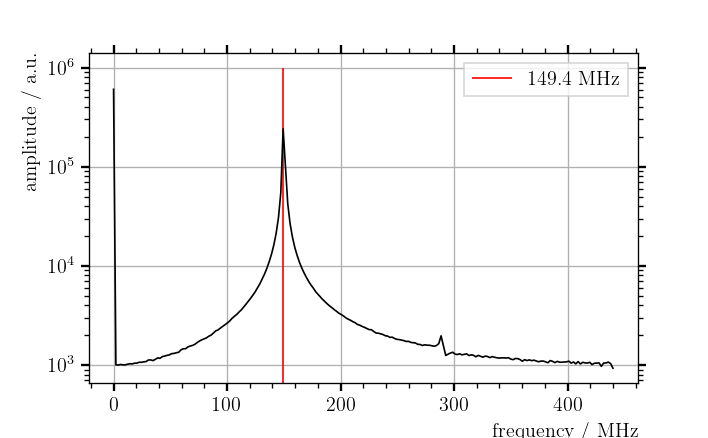
\includegraphics[width=1.\textwidth]{pictures/gandalf_23_input_ch0}
	\caption[FFT of a \SI{150}{\mega\hertz} sin signal recorded with a GANDALF module.]{The \ac{fft} of a \SI{150}{\mega\hertz} sin signal recorded with the \ac{gandalf} module 23. The peak frequency is masured to \SI{149.4(10)}{\mega\hertz}}
	\label{fig:input_offset_b2_ch0}
\end{figure}


%To test if the bits in the \acp{adc} are working, the amplitudes of all samples of every waveforms in a measurement were put into histogram.





\section{Input Offset Voltage}
The first measurement with the \ac{emusic} board is to find out the input offset voltage of the \ac{emusic} for different \ac{dac} values.
This needs to be done to determine the correct overvoltage of the \acp{sipm}, which influences among other things the gain of the \acp{sipm}.
In order to perform this measurement, the setup in \autoref{fig:input_offset_setup} was assembled.
%The \ac{emusic} board was powered by the \SI{8}{\volt} power supply and the XXXXXXXX power supply was used to supply the high voltage.
The high voltage was set to \SI{4.7}{\volt} since it was not important for the high voltage to be over the breakdown voltage of the \acp{sipm}.
It should only be over the maximum input offset the \ac{emusic} can generate for the resulting voltage to be applied in reverse direction to the \acp{sipm}.
For this measurement the \ac{emusic}s input \ac{dac} settings, which can range from 0 to \SI{511}{\dacu}, were set to \SI{0}{\dacu}.
Then the voltages between the negative high voltage pole and the voltage on the cathode of the \acp{sipm} were measured.
As measurement point for the cathode voltage, the \SI{0}{\ohm} resistor placed on the back of the \ac{sipm} board was chosen.
It is shown in \autoref{fig:meas_input_resistor}.
This measurement was done for one \ac{sipm} of each \ac{sipm} group.
The chosen \ac{sipm} were 1, 6, 11, 16, 21, 26, 31 and 36.
After measuring the different voltages, the \ac{dac} setting was increased in steps of \SI{50}{\dacu} up to \SI{500}{\dacu} and at each step the measurement was repeated.
In the following first the measurement results of the individual channels over all tested \ac{dac} settings are presented.
Afterwards, the input offset voltages of the different channels for the same setting are compared.

As an example, the measurements of all eleven tested \ac{dac} settings done with the \ac{emusic} board 2 and channel 0 are shown in \autoref{fig:input_offset_b2_ch0}.
In the upper part of the plot, the measured voltages are plotted and for the measurements with a \ac{dac} setting between \SI{100}{\dacu} and \SI{450}{\dacu} a linear fit was performed.
The first two measured voltages were not included, since they visibly do not follow the linear trend.
For all channels the first two measured values are at around \SI{1530}{\milli\volt} which indicates a constant offset voltage below \SI{100}{\adcu}.
Depending on the \ac{emusic} board and the channel also the last measured voltages were excluded from the fit since they do not follow strictly the linear trend and increase on some \ac{emusic} channels to \SI{940}{\milli\volt}.
The resulting slope and offset of the linear fit are
\begin{align}
    V_\text{offset, fit} &= \SI{-3.438(28)}{\milli\volt\per\dacu}\cdot x+\SI{1830(8)}{\milli\volt}
\end{align}
where x is the setting of the \ac{dac} in \si{\dacu}.
The bottom of the plot shows the residual plot where the difference between the linear fit and the measured values is shown.
The range on the input-offset-axis is fixed to \SIrange{-20}{20}{\milli\volt}.
In \autoref{tab:input_offset_linear_fit} the fit results for the measurements with the \ac{emusic} boards 2 and 6 are listed.
The \ac{dac} voltages of the channels differ to other channels on the same board as well as to the channels on the other board.
Therefore the measurement of the input voltage should be done for every \ac{emusic} board.
\begin{figure}
	\centering
	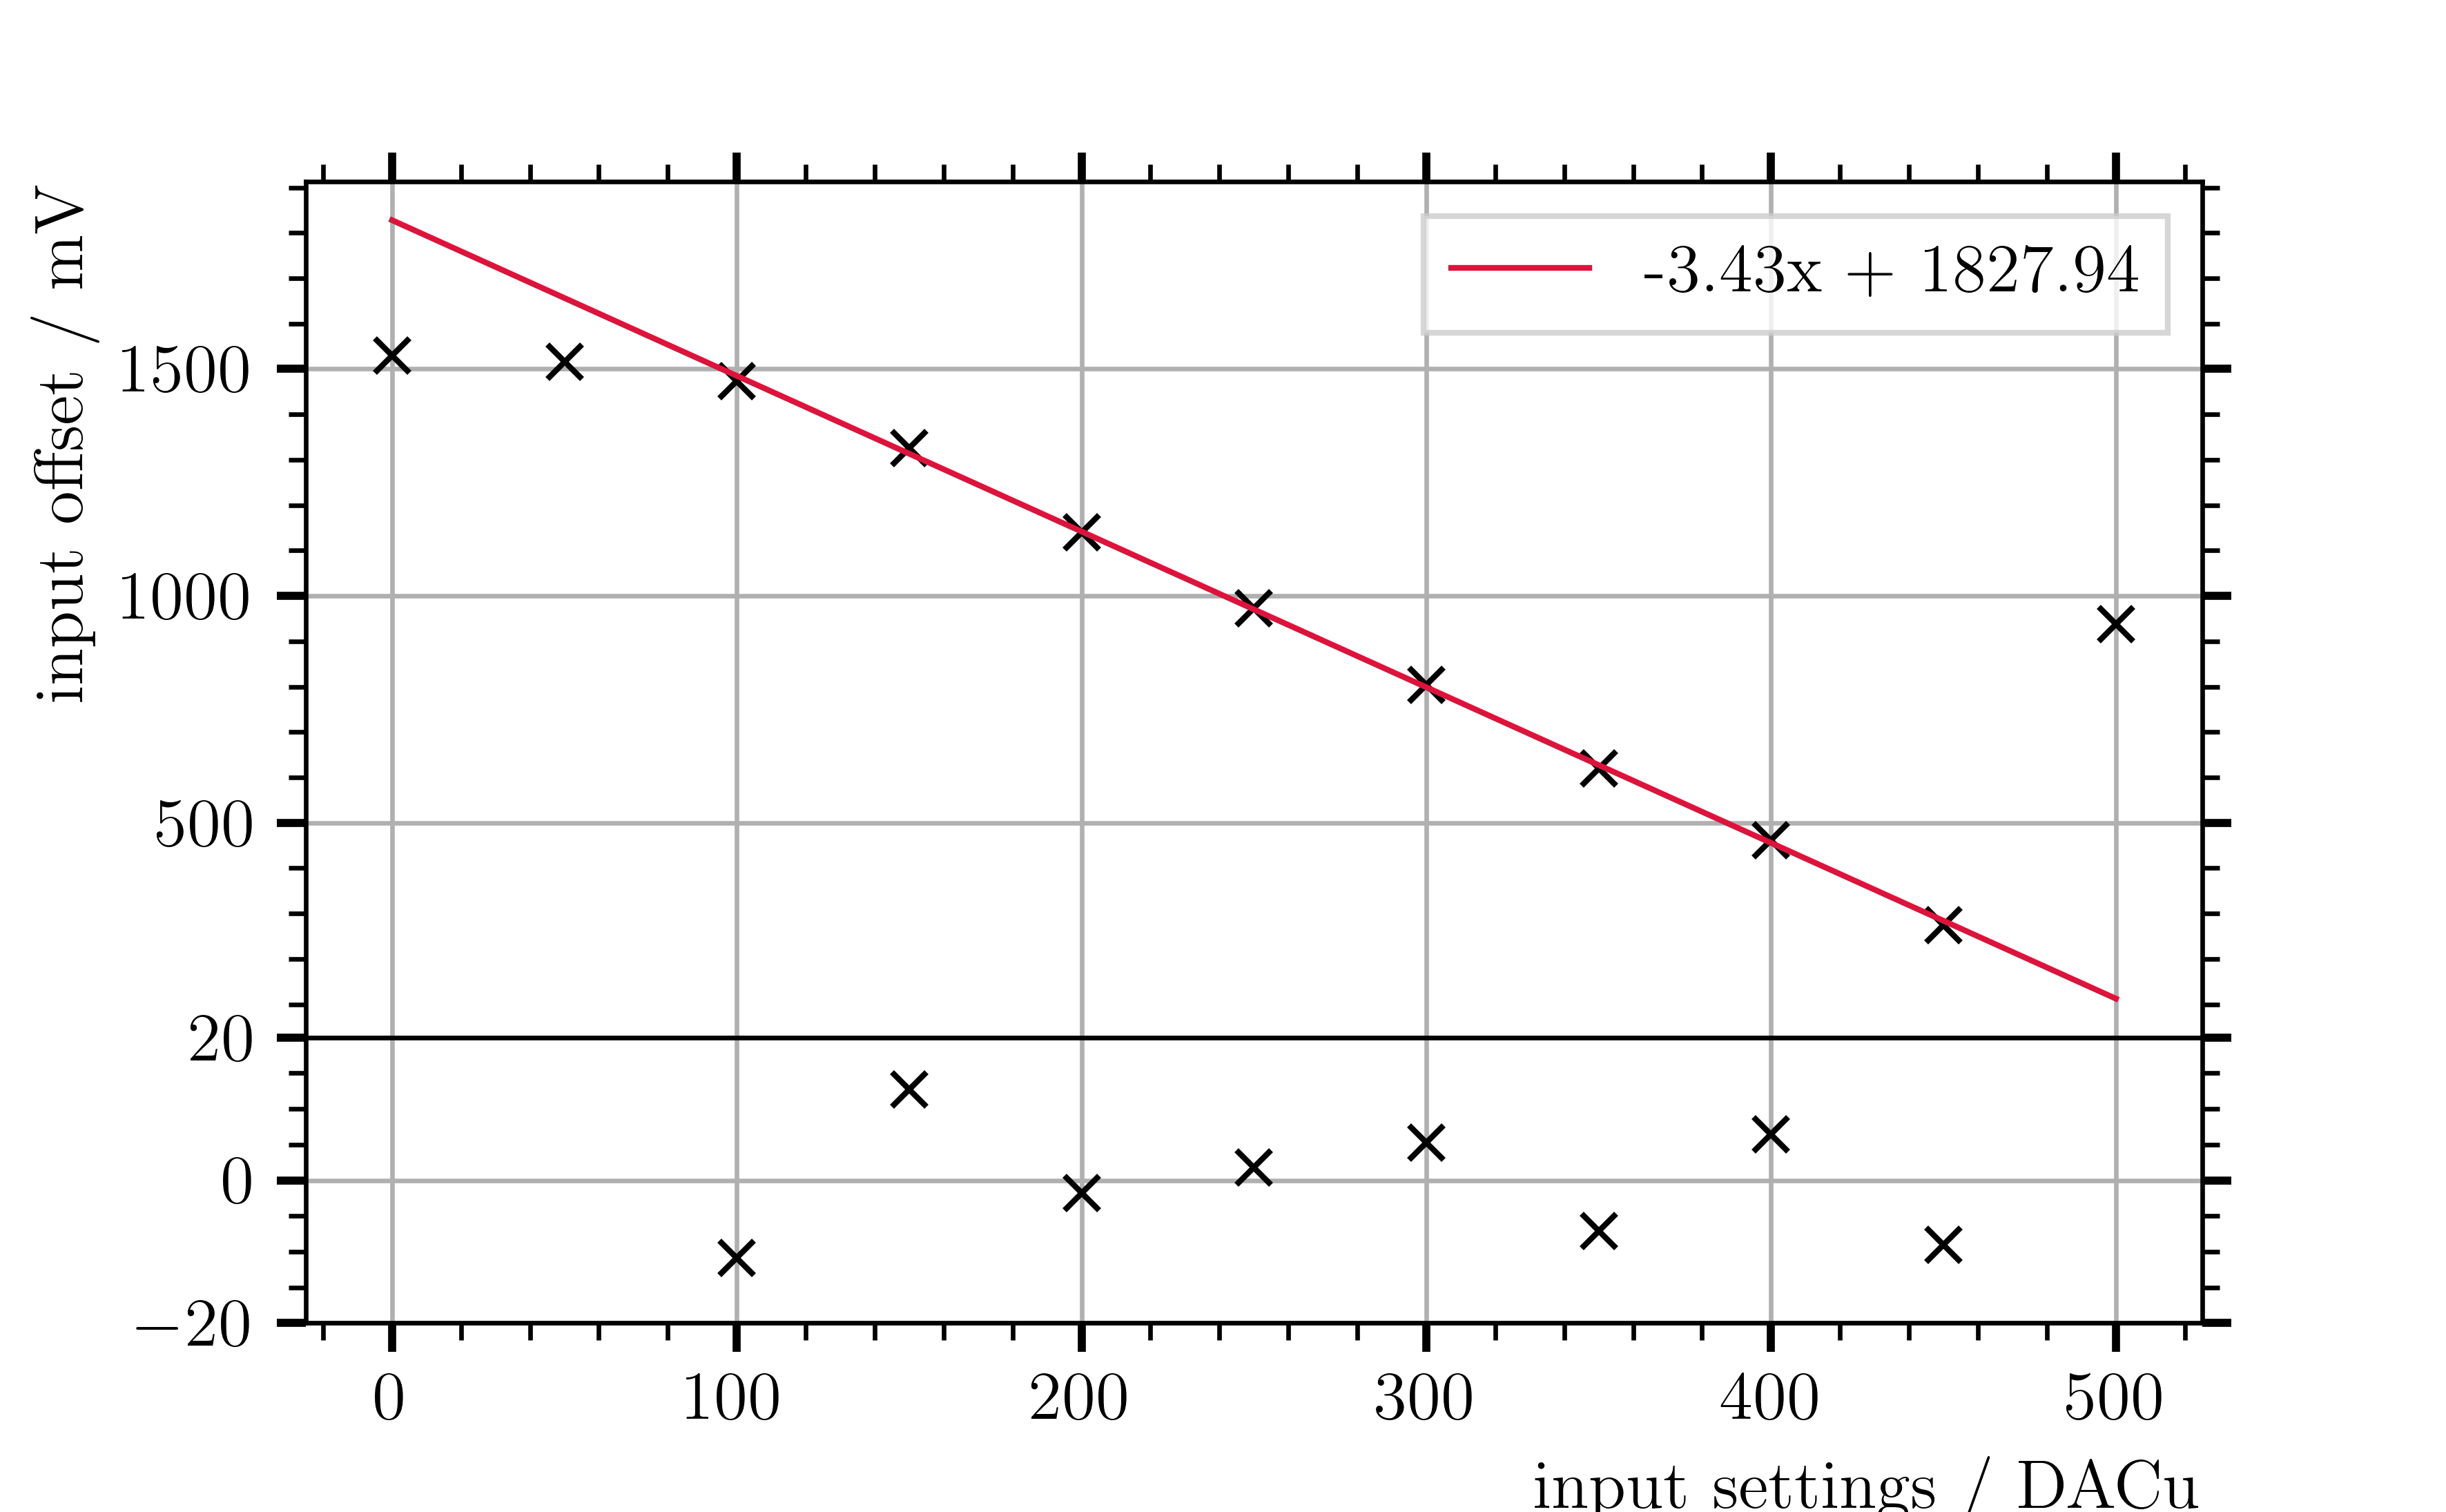
\includegraphics[width=1.\textwidth]{pictures/input_offset_board_2_channel_0}
	\caption[Input offset measurement for eMUSIC board 2 channel 1]{Input offset measurement for the channel 0 of the \ac{emusic} board 2. The input voltage was measured for input \ac{dac} settings from \SIrange{0}{500}{\dacu} in \SI{50}{\dacu} steps. A linear fit was performed for the measurements with \ac{dac} settings between \SI{100}{\dacu} and \SI{450}{\dacu}. The other measured voltages were excluded form the fit since they do not follow the linear trend. Below is the residual plot with a fixed y-axis window from \SI{-20}{\milli\volt} to \SI{-20}{\milli\volt}.}
	\label{fig:input_offset_b2_ch0}
\end{figure}
\begin{table}
	\centering
	\caption[Input offset voltages fit]{The result of fitting a linear function to the input offset measurements of the \ac{emusic} boards 2 and 6.}
	\label{tab:input_offset_linear_fit}
	\renewcommand{\arraystretch}{1.3}
	\begin{tabular*}{\textwidth}{%
		@{\extracolsep{\fill}\hspace{\tabcolsep}}
		c
		c
		S[table-format=1.3(2),table-column-width=0.20\textwidth]
		S[table-format=4.0(3),table-column-width=0.20\textwidth]
		}
		\toprule
		\ac{emusic} board & channel & {slope / \si{\milli\volt\per\dacu}} & {offset / \si{\milli\volt}} \\
		\midrule
		\multirow{8}{*}{2} & 0				& -3.438(28) & 1830(8)  \\
		                   & 1				& -3.405(15) & 1818(5)  \\
		                   & 2				& -3.377(16) & 1803(5)  \\
		                   & 3				& -3.336(17) & 1778(5)  \\
		                   & 4				& -3.290(18) & 1764(5)  \\
		                   & 5				& -3.316(20) & 1758(6)  \\
		                   & 6				& -3.211(19) & 1716(6)  \\
		                   & 7				&  &   \\
		                   & mean of all channels	& -3.163(16) & 1702(5)  \\\midrule
		\multirow{8}{*}{6} & 0				& -3.472(19) & 1843(5)  \\
		                   & 1				& -3.353(29) & 1804(9)  \\
		                   & 2				& -3.368(28) & 1795(8)  \\
		                   & 3				& -3.389(30) & 1801(9)  \\
		                   & 4				& -3.260(50) & 1747(12) \\
		                   & 5				& -3.202(33) & 1729(10) \\
		                   & 6				& -3.275(15) & 1756(4)  \\
		                   & 7				& -3.263(24) & 1749(7)  \\
		                   & mean of all channels	&  &   \\
		\bottomrule
	\end{tabular*}
	\renewcommand{\arraystretch}{1}
\end{table}

To compare the differences between channels with the same \ac{dac} settings, for three different settings the input voltage was plotted for all eight channels in \autoref{fig:input_offset_b2_dac}, \autoref{fig:input_offset_b2_dac}, and \autoref{fig:input_offset_b2_dac}.
For settings at \SI{50}{\dacu} and below, the input offset voltage is pretty equal between the channels and only differs in the single \si{\milli\volt} range around \SI{0}{\milli\volt}.
A similiar behavior is seen for \ac{dac} settings at and above \SI{500}{\dacu}, for which the input voltage is around \SI{940}{\milli\volt} and the differences between the channels is also in the single \si{milli\volt} range.
But in the \si{\dacu} range where the linear progression can be seen, the variations between the channels is larged, in some cases over \SI{70}{\milli\volt}.
This confirms, that calibration measurements of the input voltage needs to be done for all \ac{emusic} boards and all channels.
\begin{figure}
	\centering
	\begin{subfigure}[b]{1.\textwidth}
		\centering
		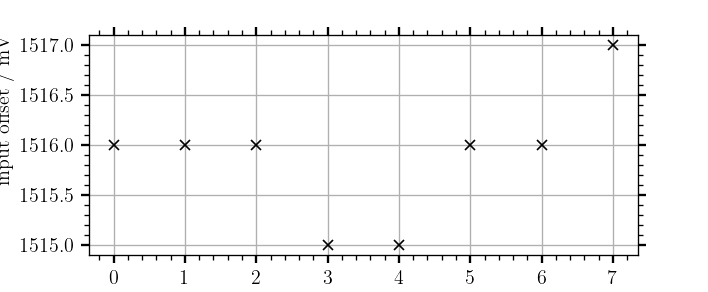
\includegraphics[width=1.\textwidth]{pictures/input_offset_b2_dac50}
		\caption{}
		\label{fig:input_offset_b2_dac50}
	\end{subfigure}
	
	\begin{subfigure}[b]{1.\textwidth}
		\centering
		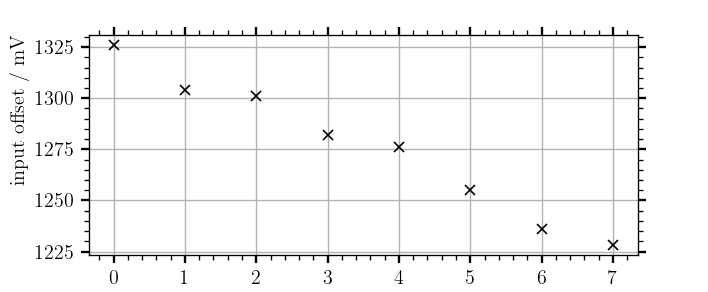
\includegraphics[width=1.\textwidth]{pictures/input_offset_b2_dac150}
		\caption{}
		\label{fig:input_offset_b2_dac150}
	\end{subfigure}

	\begin{subfigure}[b]{1.\textwidth}
		\centering
		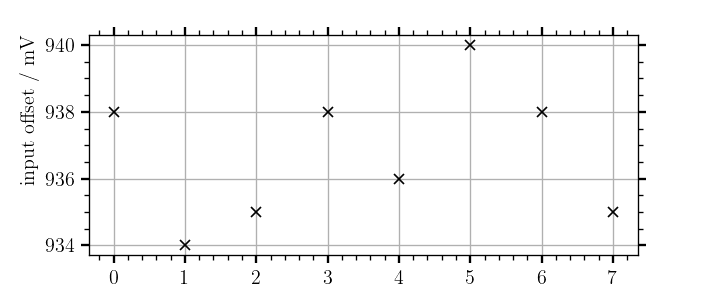
\includegraphics[width=1.\textwidth]{pictures/input_offset_b2_dac500}
		\caption{}
		\label{fig:input_offset_b2_dac500}
	\end{subfigure}
	\caption[Input offset voltage of all channels for differen \ac{dac} settings]{The input offset voltages of the different channels for the input \ac{dac} settings 50, 150, and 500. The shown meausrements were done with the \ac{emusic} board 2. While the differences between the channels for the setting 50 and 500 are less than \SI{10}{\milli\volt}, the maximum difference measured with the setting 150 is around \SI{100}{\milli\volt}.}
	\label{fig:input_offset_b2_dac}
\end{figure}

After these measurements were done, for the \ac{emusic} boards 2 and 6 the settings for which all channels have \SI{1}{\volt} offset were determined.
The resulting \ac{dac} settings and the corresponding input voltages are listed in \autoref{tab:input_offset_equalized}.
With these settings the measurement of the pole-zero cancellation and the low and high trans-impedance and pole-zero attenuation were performed.
Which are presented in the following sections.
\begin{table}
	\centering
	\caption[\ac{emusic} \ac{dac} settings for equal overvoltage between channels.]{The \ac{dac} settings for the \ac{emusic} boards 2 and 6 with which the input offset voltage is as near to \SI{1}{\volt} as possible. The uncertainties of the measured voltages is estimated from the fluctuations during the measurement to be \SI{1}{\milli\volt}.}
	\label{tab:input_offset_equalized}
	\renewcommand{\arraystretch}{1.3}
	\begin{tabular*}{\textwidth}{%
		@{\extracolsep{\fill}\hspace{\tabcolsep}}
		c
		c
		S[table-format=3.0,table-column-width=0.25\textwidth]
		S[table-format=3.1(3),table-column-width=0.25\textwidth]
		}
		\toprule
		\ac{emusic} board & channel & {\ac{dac} setting / \si{\dacu}} & {input offset / \si{\milli\volt}} \\
		\midrule
		\multirow{8}{*}{2} & 0 &   0 & 1003 \\
		                   & 1 &  50 & 1001 \\
		                   & 2 & 100 & 1003 \\
		                   & 3 & 150 & 1004 \\
		                   & 4 & 200 & 1003 \\
		                   & 5 & 250 & 1002 \\
		                   & 6 & 300 & 1002 \\
		                   & 7 & 350 & 1002 \\\midrule
		\multirow{8}{*}{6} & 0 &   0 &  999 \\
		                   & 1 &  50 &  998 \\
		                   & 2 & 100 &  997 \\
		                   & 3 & 150 & 1003 \\
		                   & 4 & 200 & 1002 \\
		                   & 5 & 250 &  995 \\
		                   & 6 & 300 &  996 \\
		                   & 7 & 350 & 1001 \\
		\bottomrule
	\end{tabular*}
	\renewcommand{\arraystretch}{1}
\end{table}

\section{Pole-Zero Cancellation Shaper}

In this section the results from the characterization of the pole-zero cancellation shaper and its effect with different settings are described.
Hereby the amplitude of the peak and the \ac{fwhm} are of interest.
The tests were done using the setup described in \autoref{sec:setup}.
The high voltage for this and all following measurements, as long as not otherwise stated, was set to \SI{43}{\volt}. 
A \ac{gandalf} module was used for the digitization.
The \ac{emusic} settings of one of these measurements are shown in \autoref{} in the appendix.
For the other measurements, only the pole-zero settings were changed.
Each measurement includes approximately \num{80000} events, for which the mean waveforms are shown in the plots below.
The values for the amplitude and \ac{fwhm} were calculated for each individual waveform and theire mean values are presented here for the different measurements.

First the pole-zero cancellation was disabled to perform measurements for a reference amplitude and \ac{fwhm}.
In \autoref{fig:pz_no_pz} the mean of all \num{80000} waveforms is shown.
The mean amplitude is 
\begin{align}
    V_{amp} &= \SI{523(46)}{\milli\volt}
\end{align}
and the \ac{fwhm} is
\begin{align}
    t_\text{FWHM} &= \SI{113(3)}{\nano\second}.
\end{align}
\begin{figure}
	\centering
	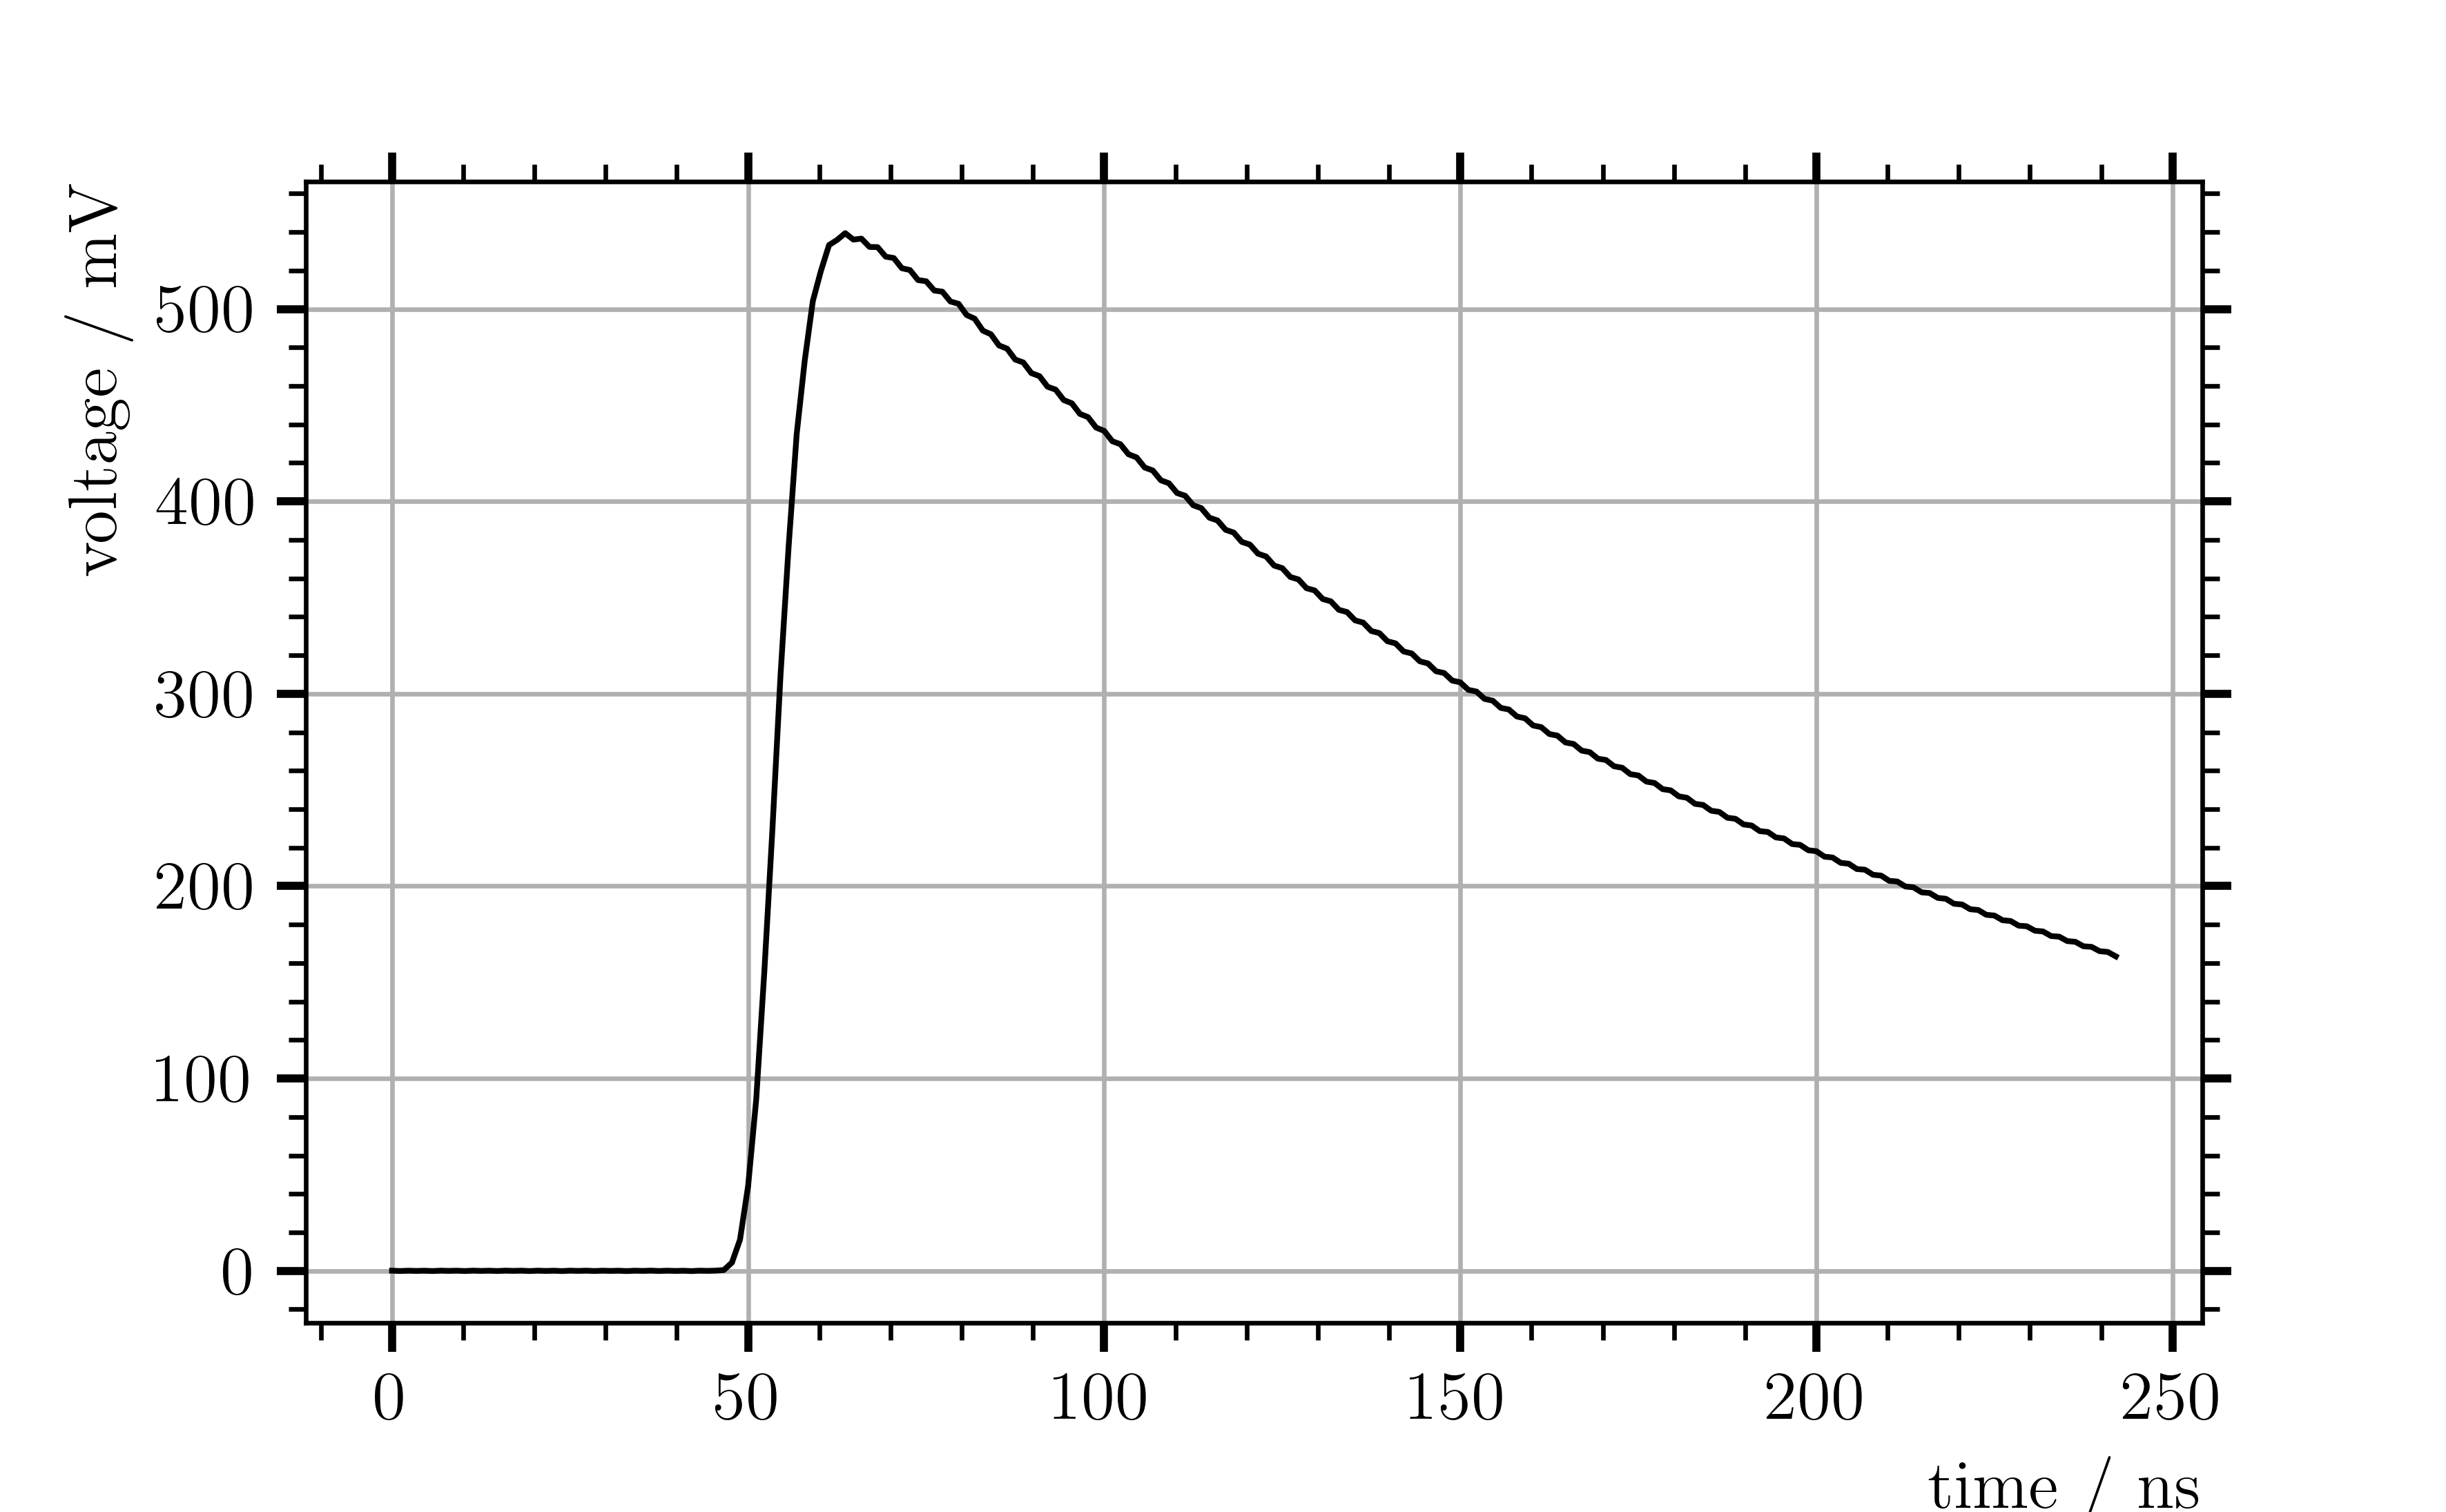
\includegraphics[width=1.\textwidth]{pictures/pz_no_pz}
	\caption[Mean waveform for a measurement without pole-zero cancellation.]{Mean waveform for a measurement without pole-zero cancellation.}
	\label{fig:pz_no_pz}
\end{figure}

Next the measurement with enabled pole-zero cancellation and with fixed settings for its capacitor and variing resistor values.
The resistor settings were changed to all possible values, from 0 to 7, and the capacitor setting was kept at 31.
\autoref{fig:pz_resistor} presents the mean waveforms for the eight measurements.
The determined amplitudes and \ac{fwhm} and the coresponding decrease in respect to the values without pole-zero cancellation are listed in \autoref{tab:pz_res_cap}.
For higher resistor values, the amplitude decreases from \SI{354(30)}{\milli\volt} for the setting 0 down to \SI{143(13)}{\milli\volt} for the setting 7.
Also the \ac{fwhm} decreases down to \SI{10.2(6)}{\nano\second} with higher resistor settings.



%Of all measurements the one with the resistor setting 0 had the highest mean amplitude with 
%\begin{align}
%    V_\text{amp,R=0} &= \SI{1(1)}{\milli\volt}
%\end{align}
%which correspondes to a amplitude attenuation of \SI{1(1)}{\percent}.
%With these settings a \ac{fwhm} of
%\begin{align}
%    t_\text{FWHM,R=0} &= \SI{1(1)}{\nano\second}
%\end{align}
%was measured, which is \SI{1(1)}{\percent} of the \ac{fwhm} measured without pole-zero cancellation.
\begin{figure}
	\centering
	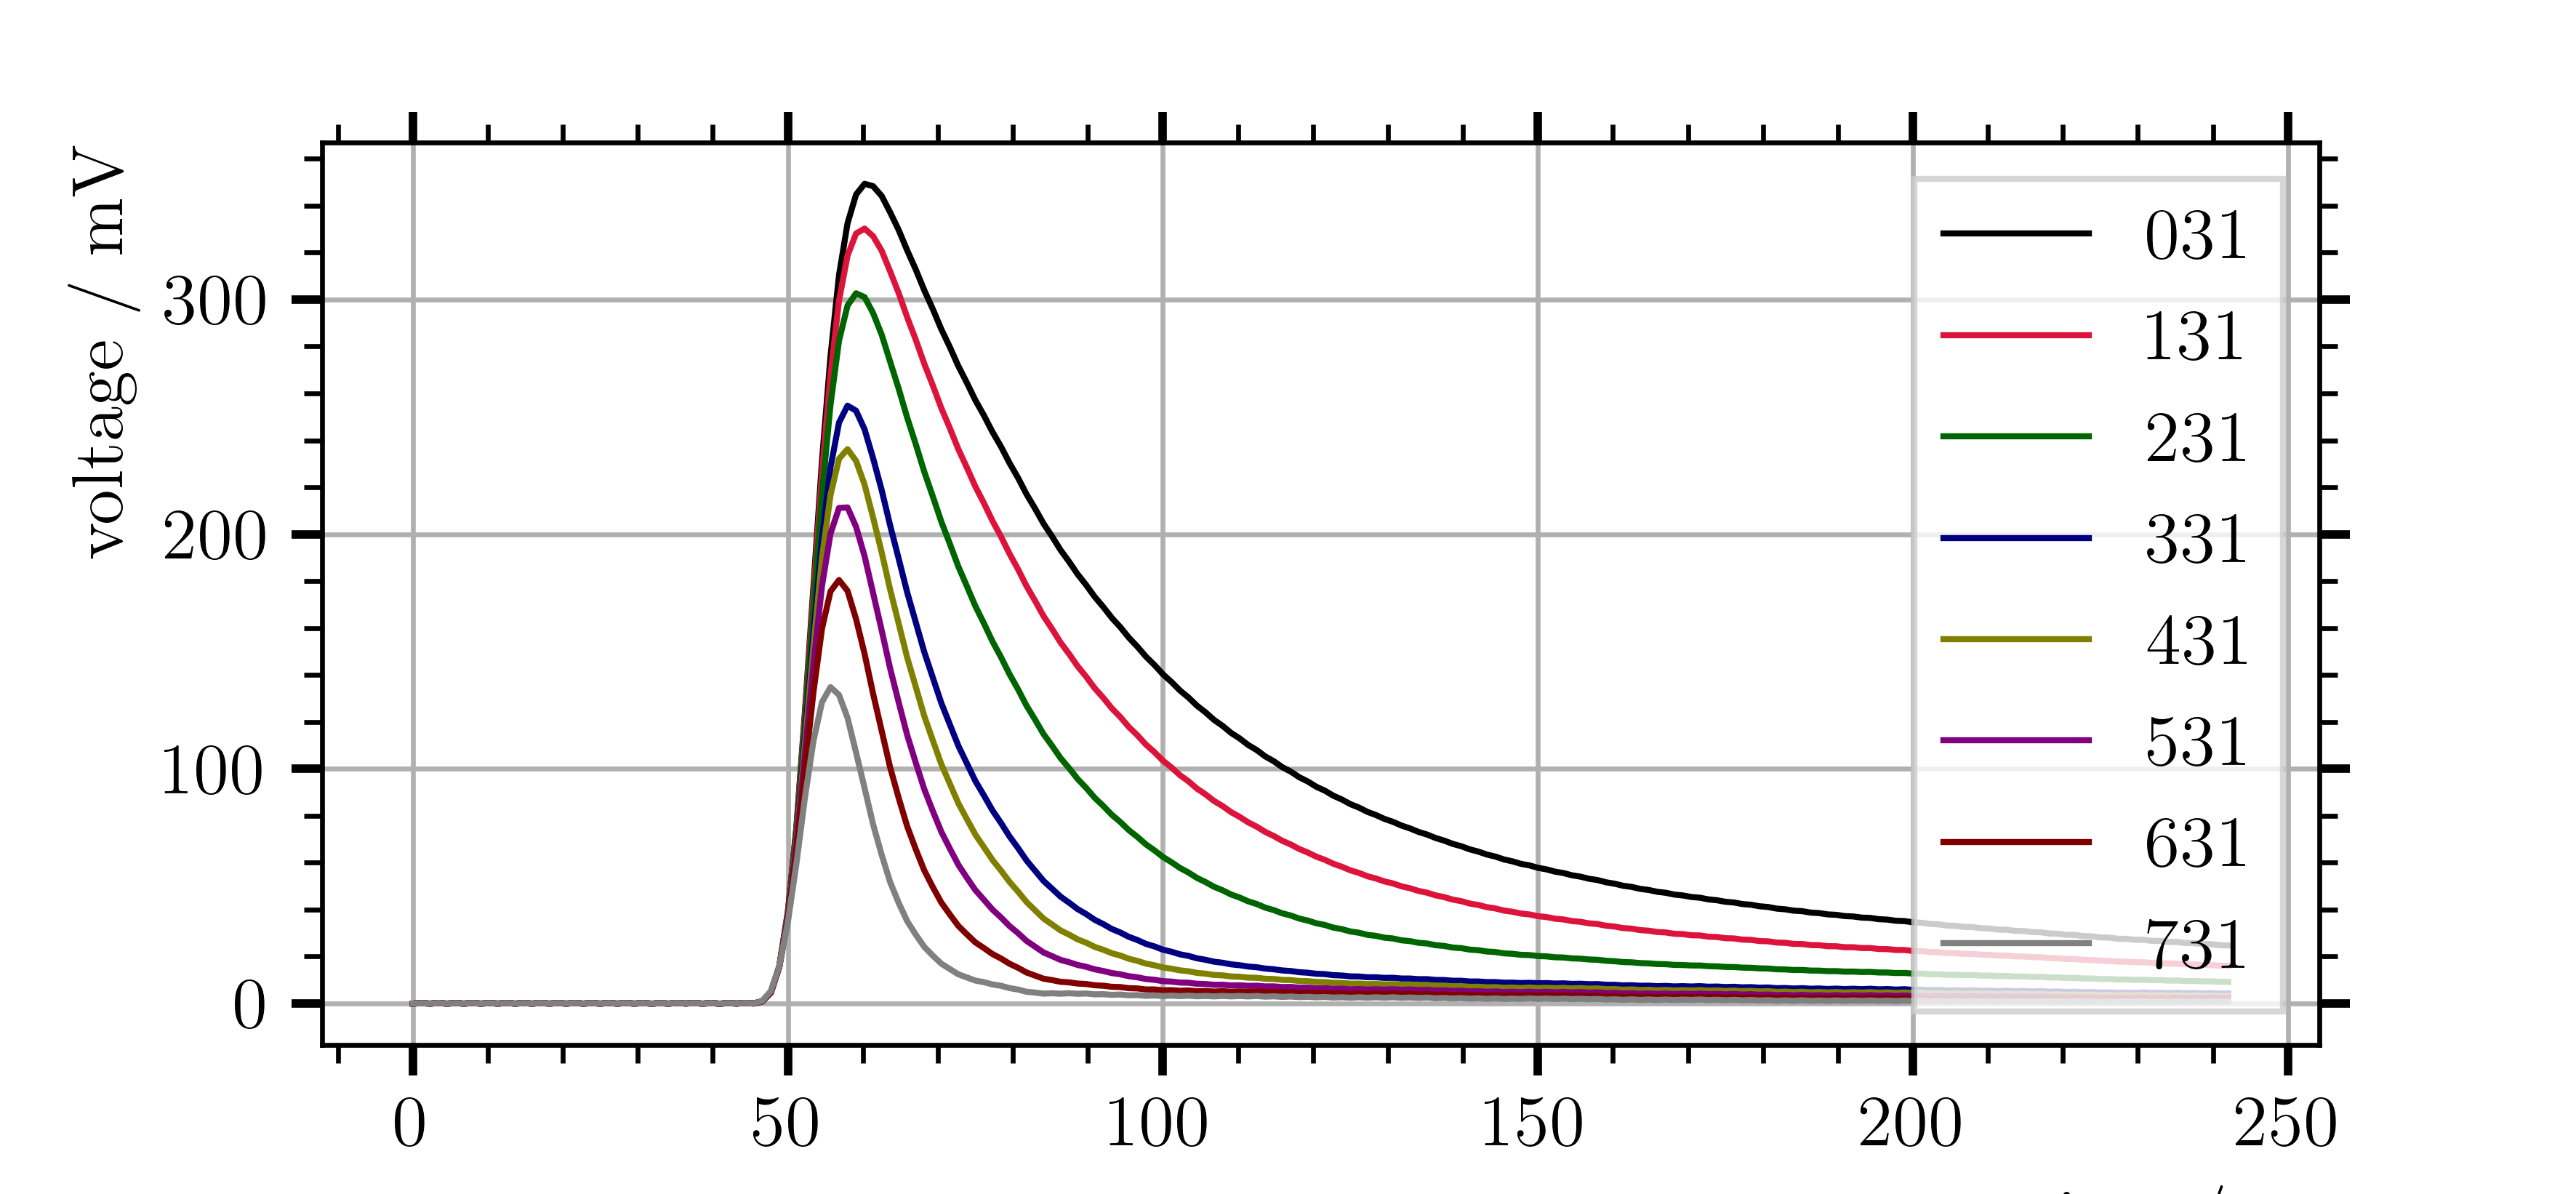
\includegraphics[width=1.\textwidth]{pictures/pz_resistor}
	\caption[Mean waveform for different pz-cancellation resistor values.]{Mean waveform for different pz-cancellation resistor values. The pole-zero cancellation capacitor setting was kept at 31. With increasing resistor settings the amplitude decreases and the width of the peak becomes smaller.}
	\label{fig:pz_resistor}
\end{figure}

The measurements with different capacitor settings were performed with the resistor setting of 0.
For the different measurements, the capacitor settings were changed to all 32 possible values, from 0 to 31.
In \autoref{tab:pz_res_cap} the mean values for the maximum amplitude and the \ac{fwhm} as well as the decrease compared to the values with disabled pole-zero cancellation are listed.
The mean waveforms for the measurements with the capacitor settings 0, 5, 10, 15, 20, 25, and 31 are shown in \autoref{fig:pz_capacitor}.
Similar to the effect of the resistor, with higher capacitor settings, the \ac{fwhm} decreases.
For the setting 0 it is \SI{58.1(27))}{\nano\second} and with the maximal setting 31 it is decreased to \SI{36.8(11)}{\nano\second}.
But, opposite to the resistor setting effects, the signal amplitude increases with higher settings up to \SI{354(30)}{\milli\volt}.
The minimal amplitude value, with the capacitor setting 0, is \SI{206(17)}{\milli\volt}.
So by adjusting the capacitor, the amplitude can be increased by a factor of \num{1.7(3)}.
\begin{figure}
	\centering
	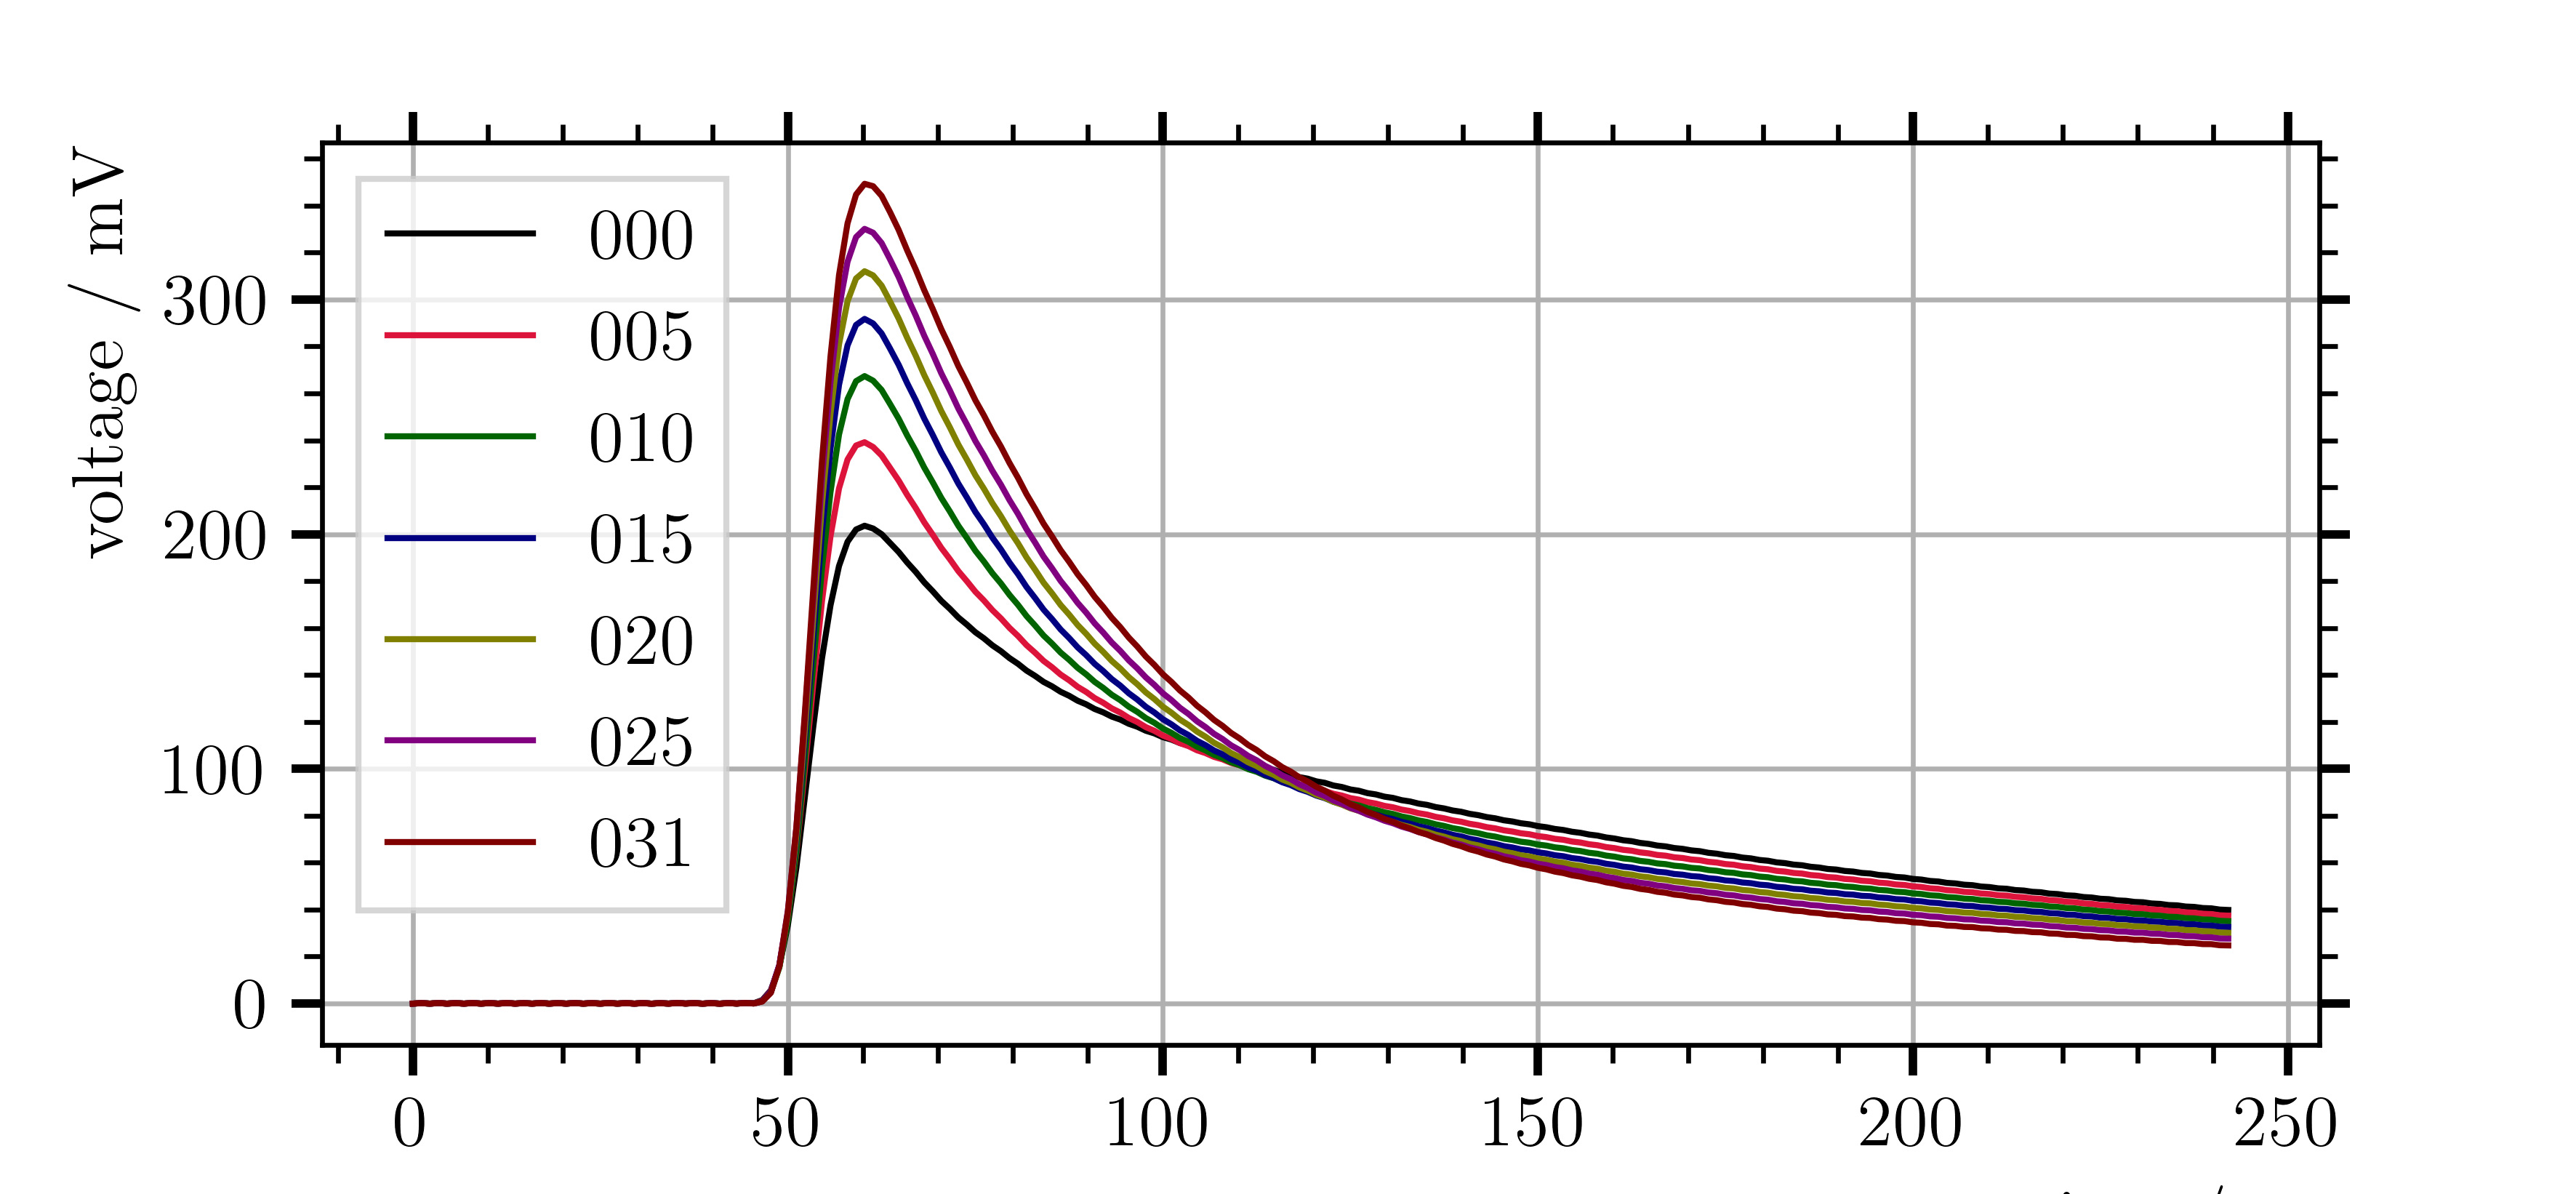
\includegraphics[width=1.\textwidth]{pictures/pz_capacitor}
	\caption[Mean waveform for different pz-cancellation capacitor values.]{Mean waveform for different pz-cancellation capacitor values. The resistor settings were kept at 0 for all of the seven measurements.}
	\label{fig:pz_capacitor}
\end{figure}

\begin{table}
	\centering
	\caption[Amplitudes and FWHMs of measured signals for different PZ settings.]{The amplitudes and \acp{fwhm} measured with different resistor and capacitor settings for the pole-zero cancellation. For each setting, around \num{80000} waveforms were recorded. The listed values are the mean amplitudes and \acp{fwhm} of all corresponding waveforms.}
	\label{tab:pz_res_cap}
	\renewcommand{\arraystretch}{1.3}
	\begin{tabular*}{\textwidth}{%
		@{\extracolsep{\fill}\hspace{\tabcolsep}}
		S[table-format=1.0,table-column-width=0.20\textwidth]
		S[table-format=2.0,table-column-width=0.20\textwidth]
		S[table-format=3.0(2),table-column-width=0.20\textwidth]
		S[table-format=3.1(3),table-column-width=0.20\textwidth]
		}
		\toprule
		{R} & {C} & {amplitude / \si{\milli\volt}} & {FWHM / \si{\nano\second}} \\
		\midrule
		{-} & {-}  & 523(46) & 113(3)   \\
		0   & 31   & 354(30) & 36.8(11) \\
		1   & 31   & 335(29) & 30.5(9)  \\
		2   & 31   & 308(27) & 24.4(8)  \\
		3   & 31   & 262(23) & 17.5(6)  \\
		4   & 31   & 243(21) & 15.7(6)  \\
		5   & 31   & 220(19) & 14.0(6)  \\
		6   & 31   & 188(17) & 12.1(5)  \\
		7   & 31   & 143(13) & 10.2(6)  \\
		0   &  0   & 206(17) & 58.1(27) \\
		0   &  5   & 242(21) & 43.2(17) \\
		0   & 10   & 271(23) & 38.7(14) \\
		0   & 15   & 296(25) & 36.9(12) \\
		0   & 20   & 316(27) & 36.5(12) \\
		0   & 25   & 334(28) & 36.4(11) \\
		0   & 31   & 354(30) & 36.8(11) \\ 
		\bottomrule
	\end{tabular*}
	\renewcommand{\arraystretch}{1}
\end{table}



\section{Transimpedance and Pole-Zero Attenuation}
After investigating the effects of the pole-zero shaper the influences between the normal and the low pole-zero attenuation settings are examined.
Also the high and low transimpedance settings are investigated.

First the pole-zero attenuation was looked at.
Therefore another measurement without the lower attenuation setting was performed.
The pole-zero cancellation resistor setting was set to R=3 and the capacitor setting was set to C=31. 
In \autoref{fig:pz331_att} the mean waveforms with and without lower attenuation are presented.
The peak of the waveform is not affected by the lower attenuation setting.
Mainly the tail is of the waveform is increased in amplitude by using the lower attenuation.
This increases the peak width, but as it can be seen in \autoref{fig:pz331_att} it can also prevent small overshoot of the signal.

The measurement was also done with the pole-zero settings 7 and 0 for the resistor and capacitor, respectively.
The result is shown in \autoref{fig:pz700_att}.
Here the same behavior can be observed.
The peak amplitude is not influenced, only the amplitude of the tail is increased by the lower attenuation.
\begin{figure}
	\centering
	\begin{subfigure}[b]{1.\textwidth}
		\centering
		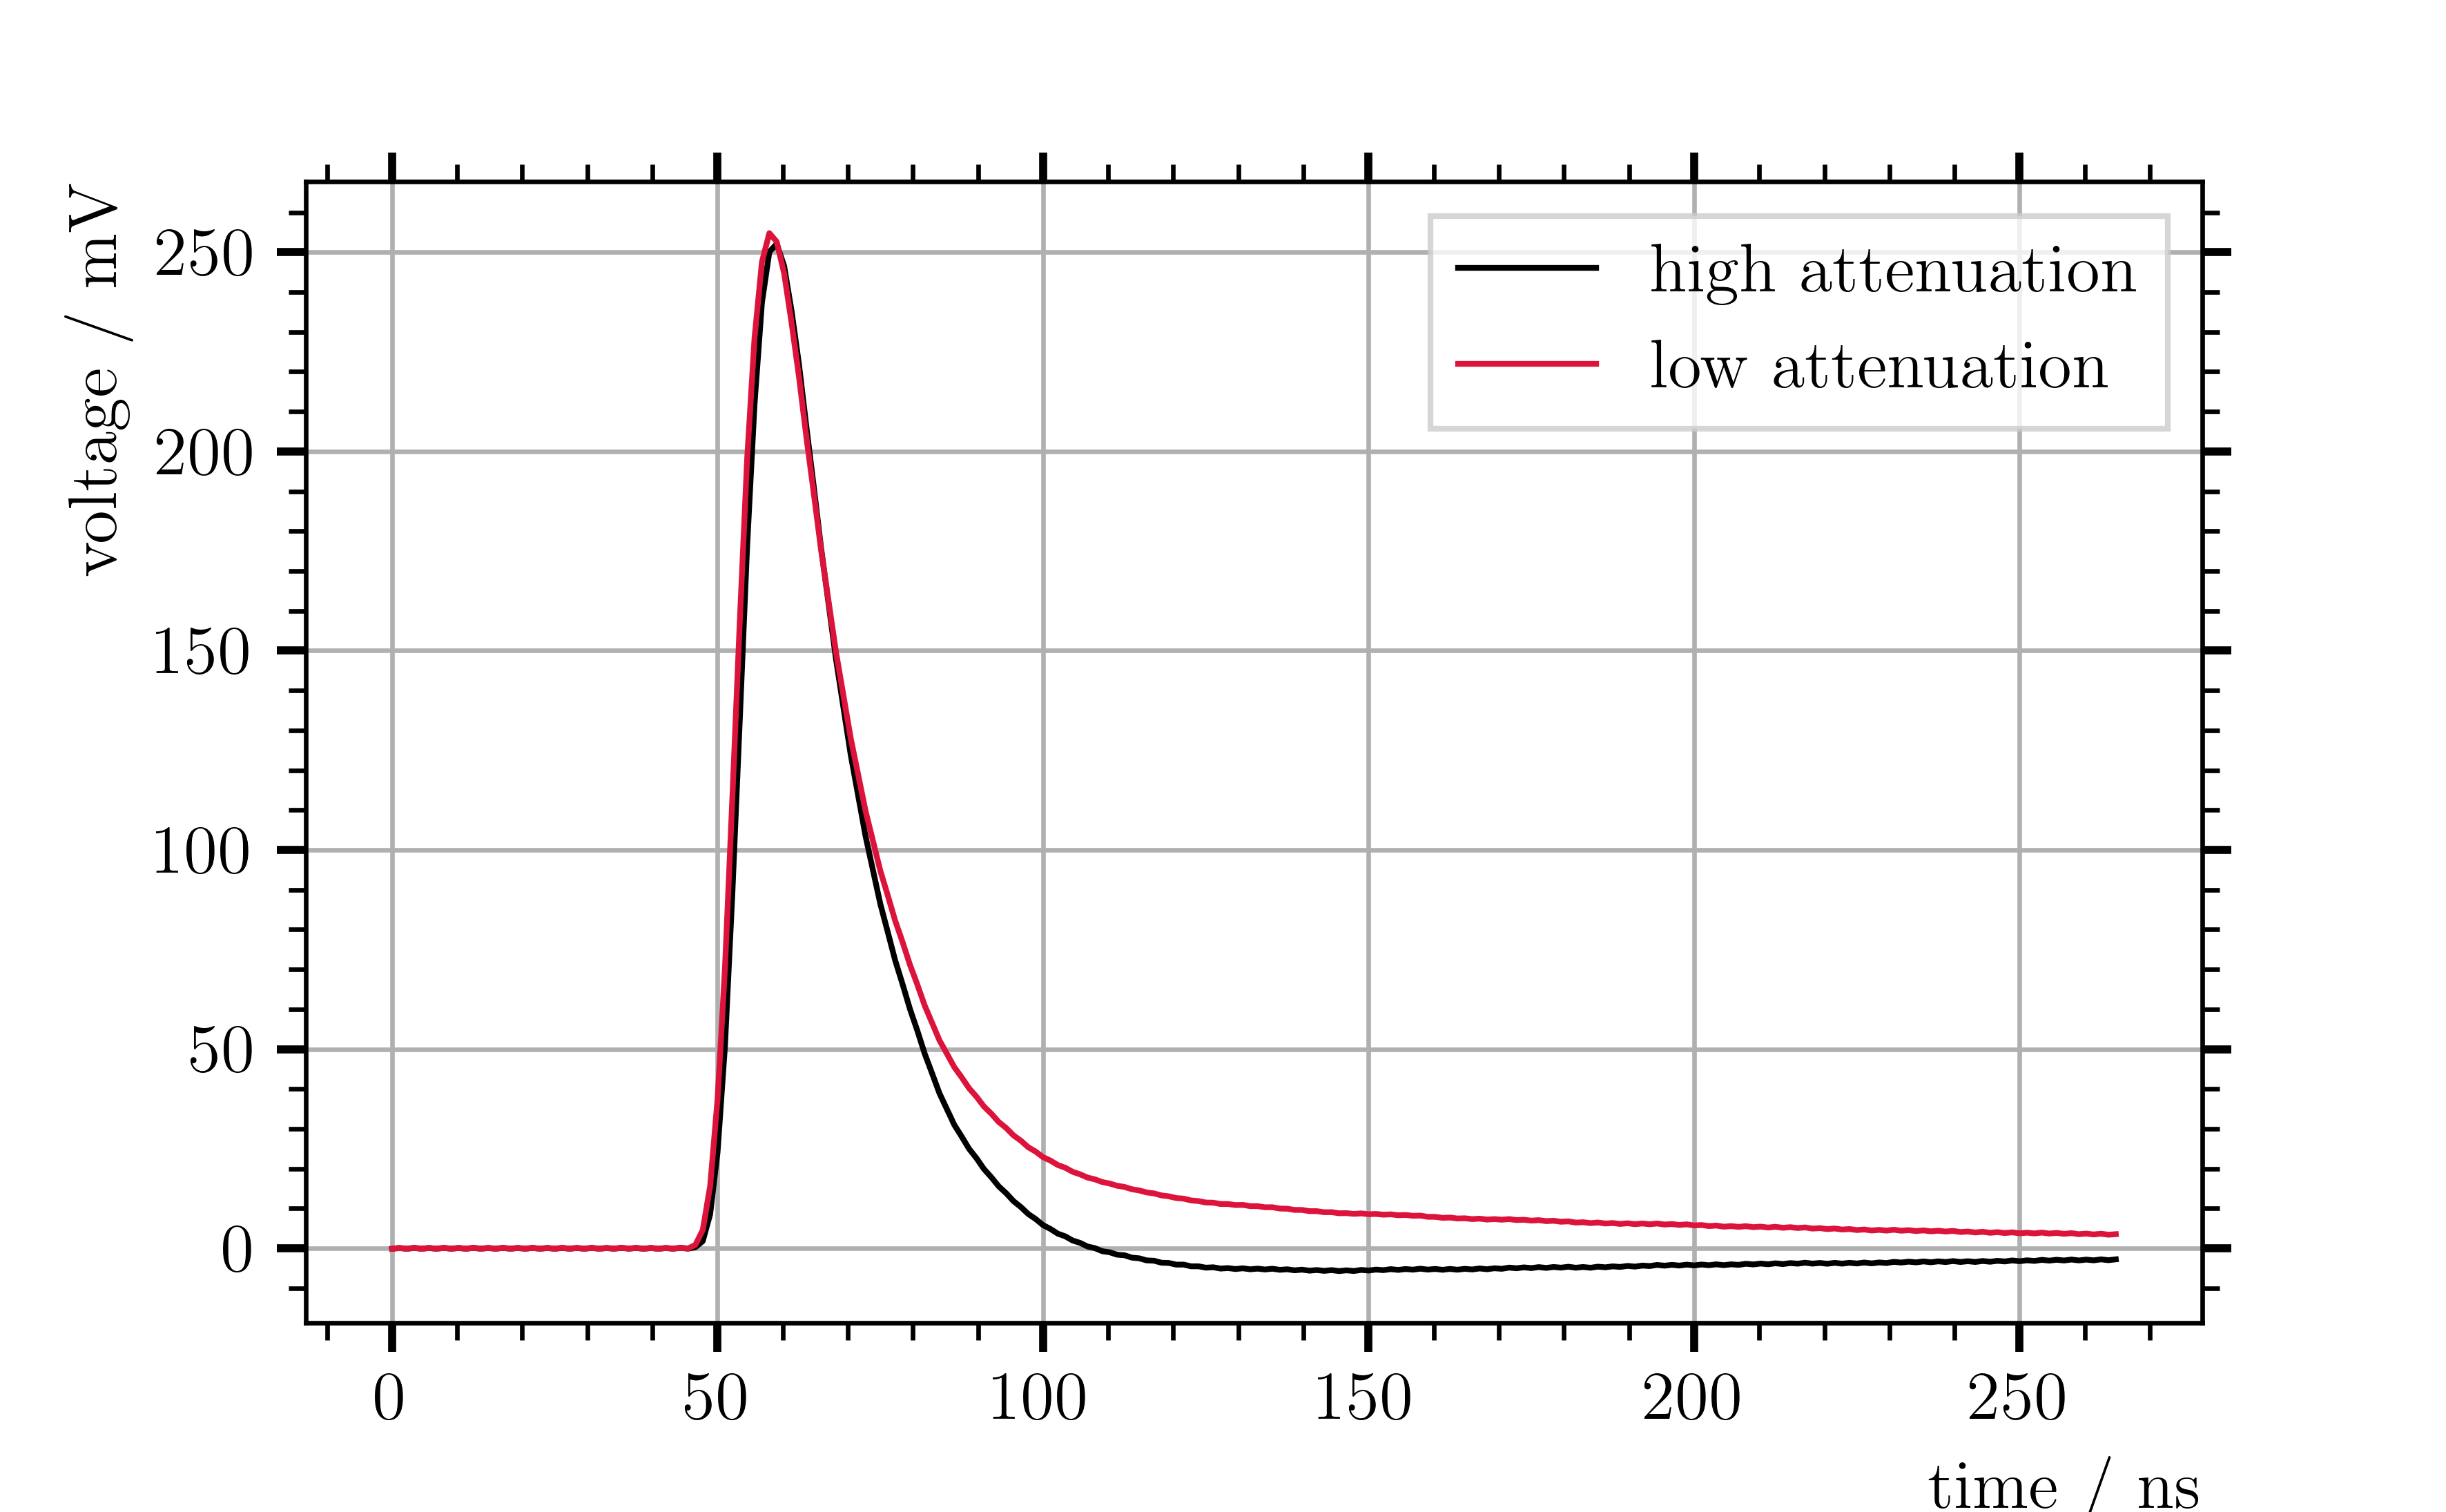
\includegraphics[width=1.\textwidth]{pictures/att_pz331}
		\caption[]{}
		\label{fig:pz331_att}
	\end{subfigure}
	\begin{subfigure}[b]{1.\textwidth}
		\centering
		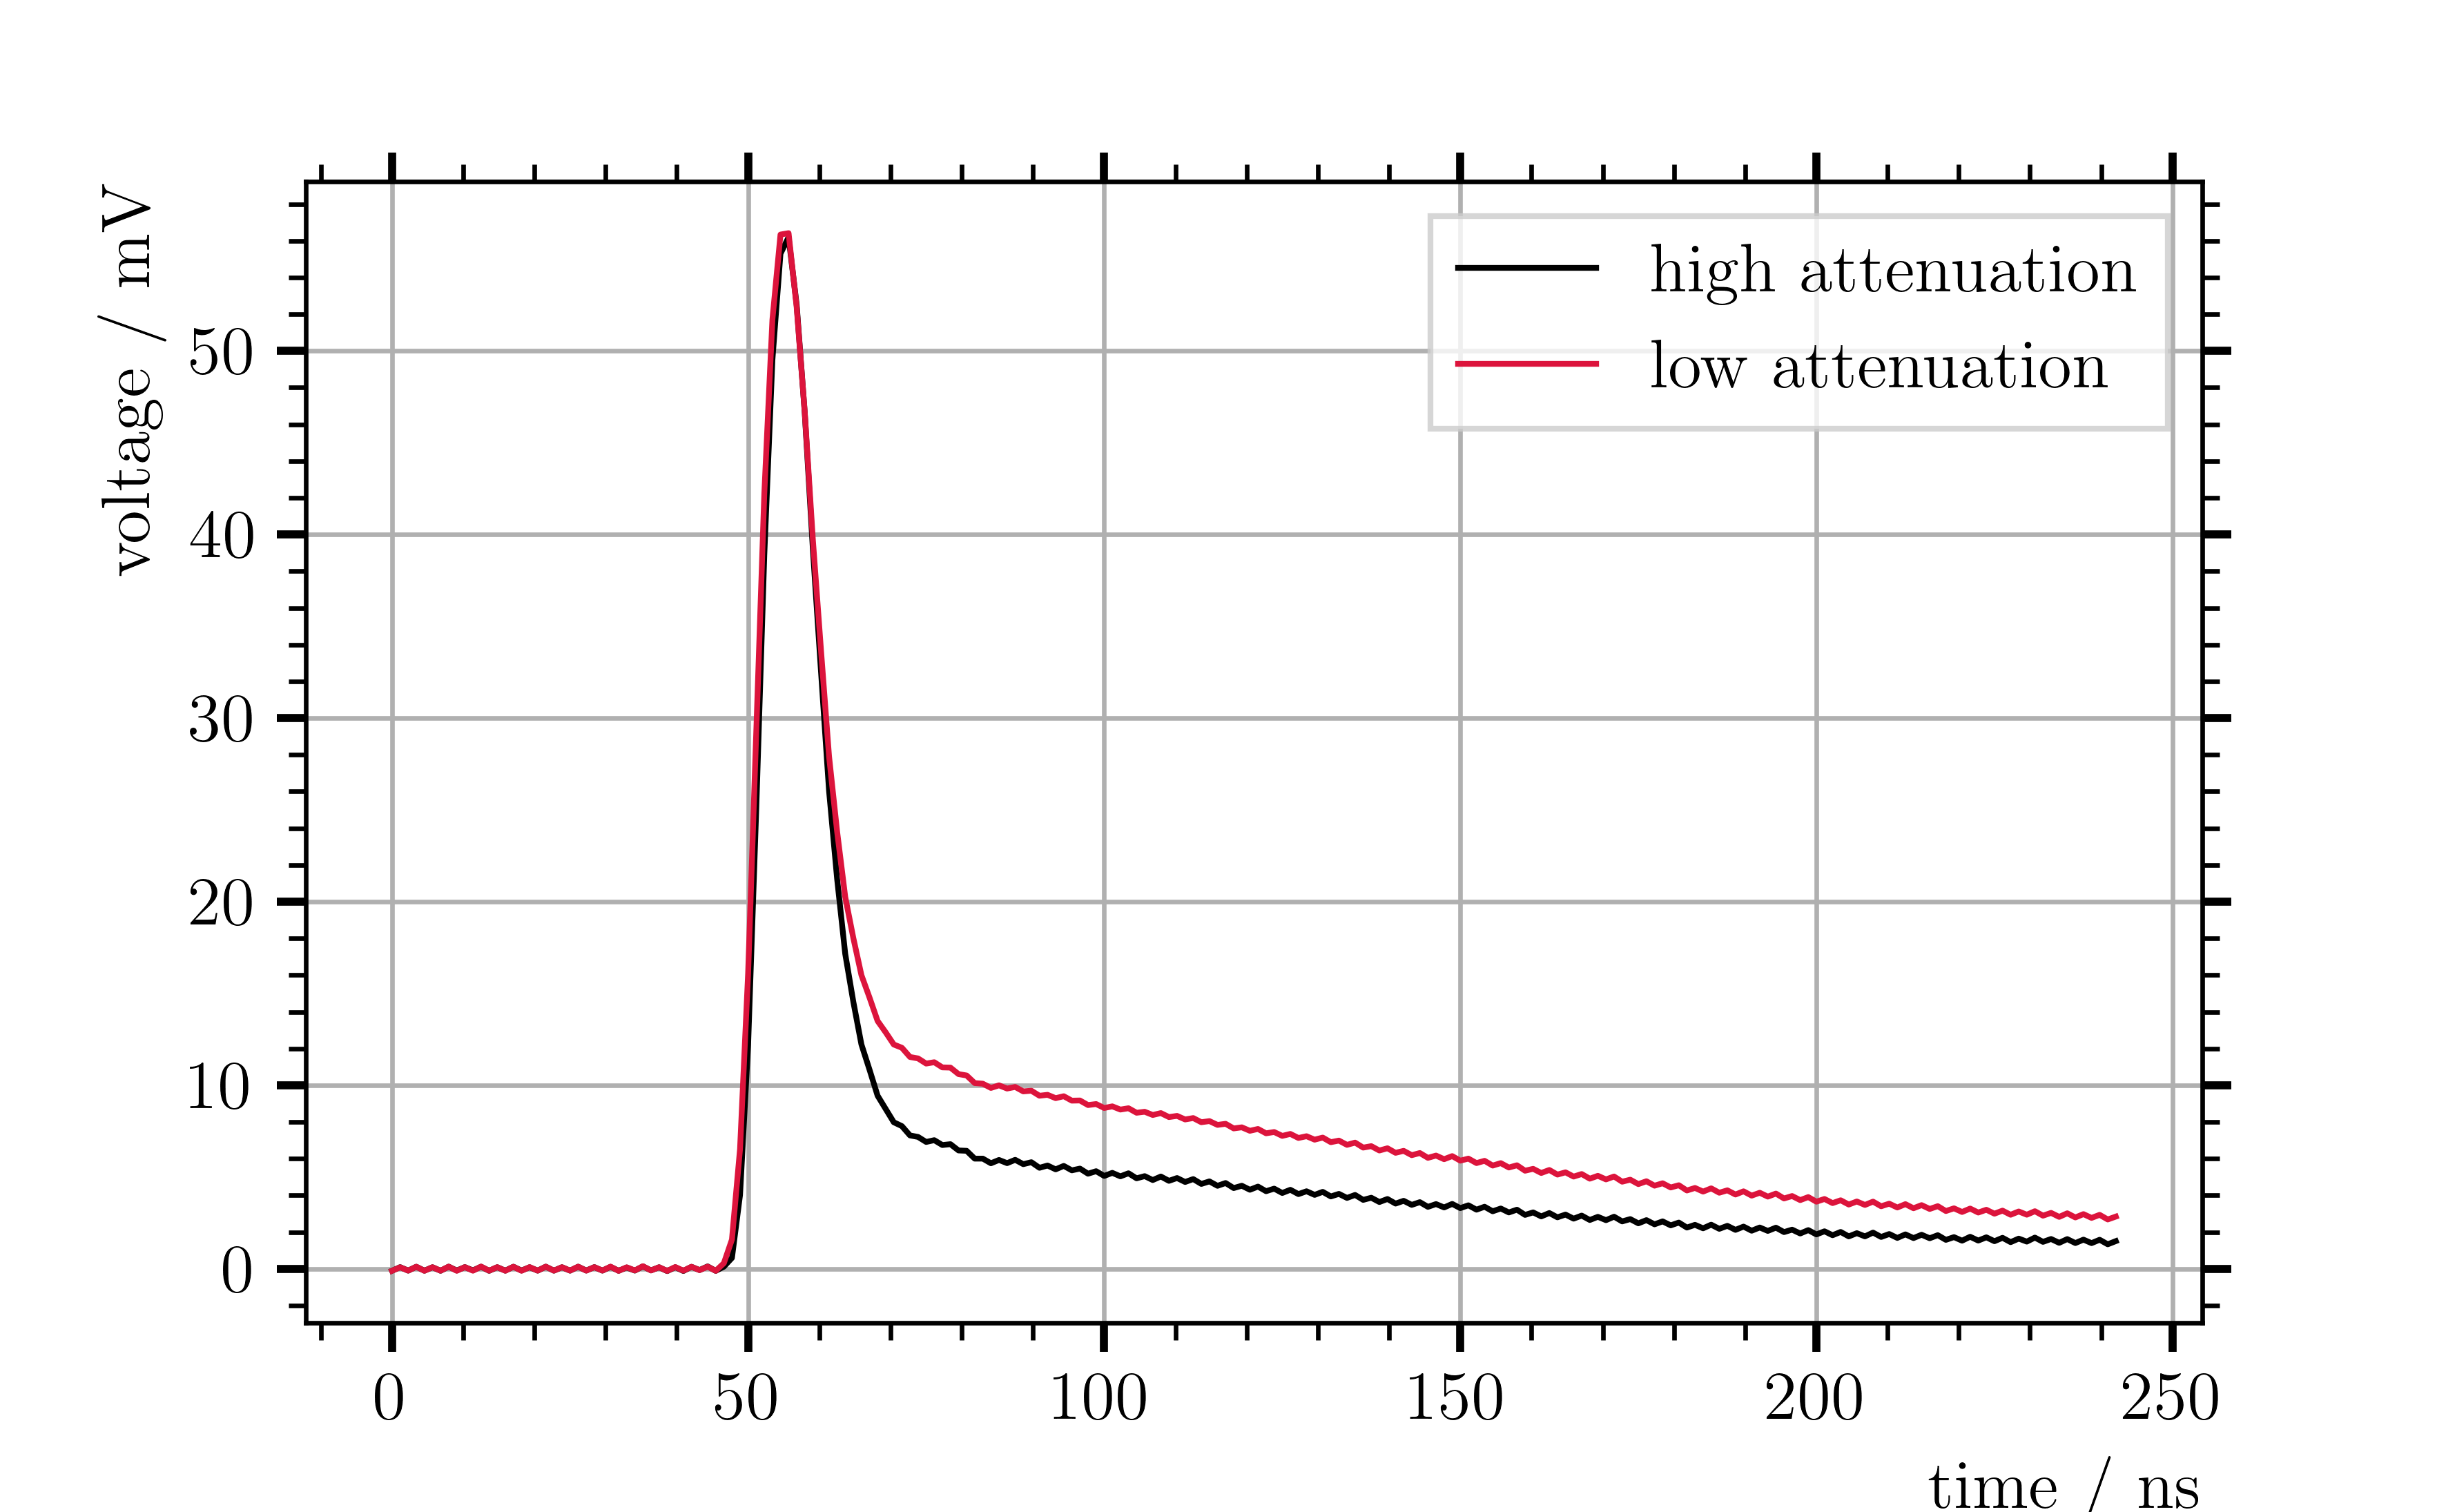
\includegraphics[width=1.\textwidth]{pictures/att_pz700}
		\caption[]{}
		\label{fig:pz700_att}
	\end{subfigure}
	\caption[Plot of the low attenuation effect with two pole-zero settings.]{The mean waveforms of two measurements, each around \num{80000} waveforms, with the pole-zero settings 7, for the resistor, and 00 for the capacitor. One measurement was done with the low attenuation option of the \ac{emusic} and the other was done without that option. Mostly the tail of the peaks is affected by the low attenuation option, while the peak amplitude seems to be not changed.}
	\label{fig:pz_att}
\end{figure}

Next, the high and low transimpedance settings were investigated.
Therefore two measurements without pole-zero cancellation were taken, one with high and a second with low transimpedance.
Again, both measurements consist of around \num{80000} waveforms.
Mean waveforms were calculated for both measurements and plotted in \autoref{fig:low_imp_wf}.
The mean amplitude of the events with high transimpedance is
\begin{align}
	V_\text{high imp} &= \SI{540(50)}{\milli\volt}
\end{align}
and of the events with low transimpedance the mean amplitude is
\begin{align}
	V_\text{low imp} &= \SI{185(14)}{\milli\volt}.
\end{align}
This results in a reduction by the factor \num{0.34(4)} if the low transimpedance is used.
The measurements were repeated with the settings 3 and 31 for the pole-zero resistor and capacitor, respectively.
The mean amplitudes for these measurements are
\begin{align}
	V_\text{high imp} &= \SI{272(22)}{\milli\volt}\\
	\text{and}\quad V_\text{low imp} &= \SI{94(7)}{\milli\volt}
\end{align}
and the factor by which the signal amplitude decreases is \num{0.35(4)}, which is also in agreement with the results of the other measurement.
The plots of the mean waveforms for the measurements with pole-zero cancellation are shown in the appendix in \autoref{}.
\begin{figure}
	\centering
	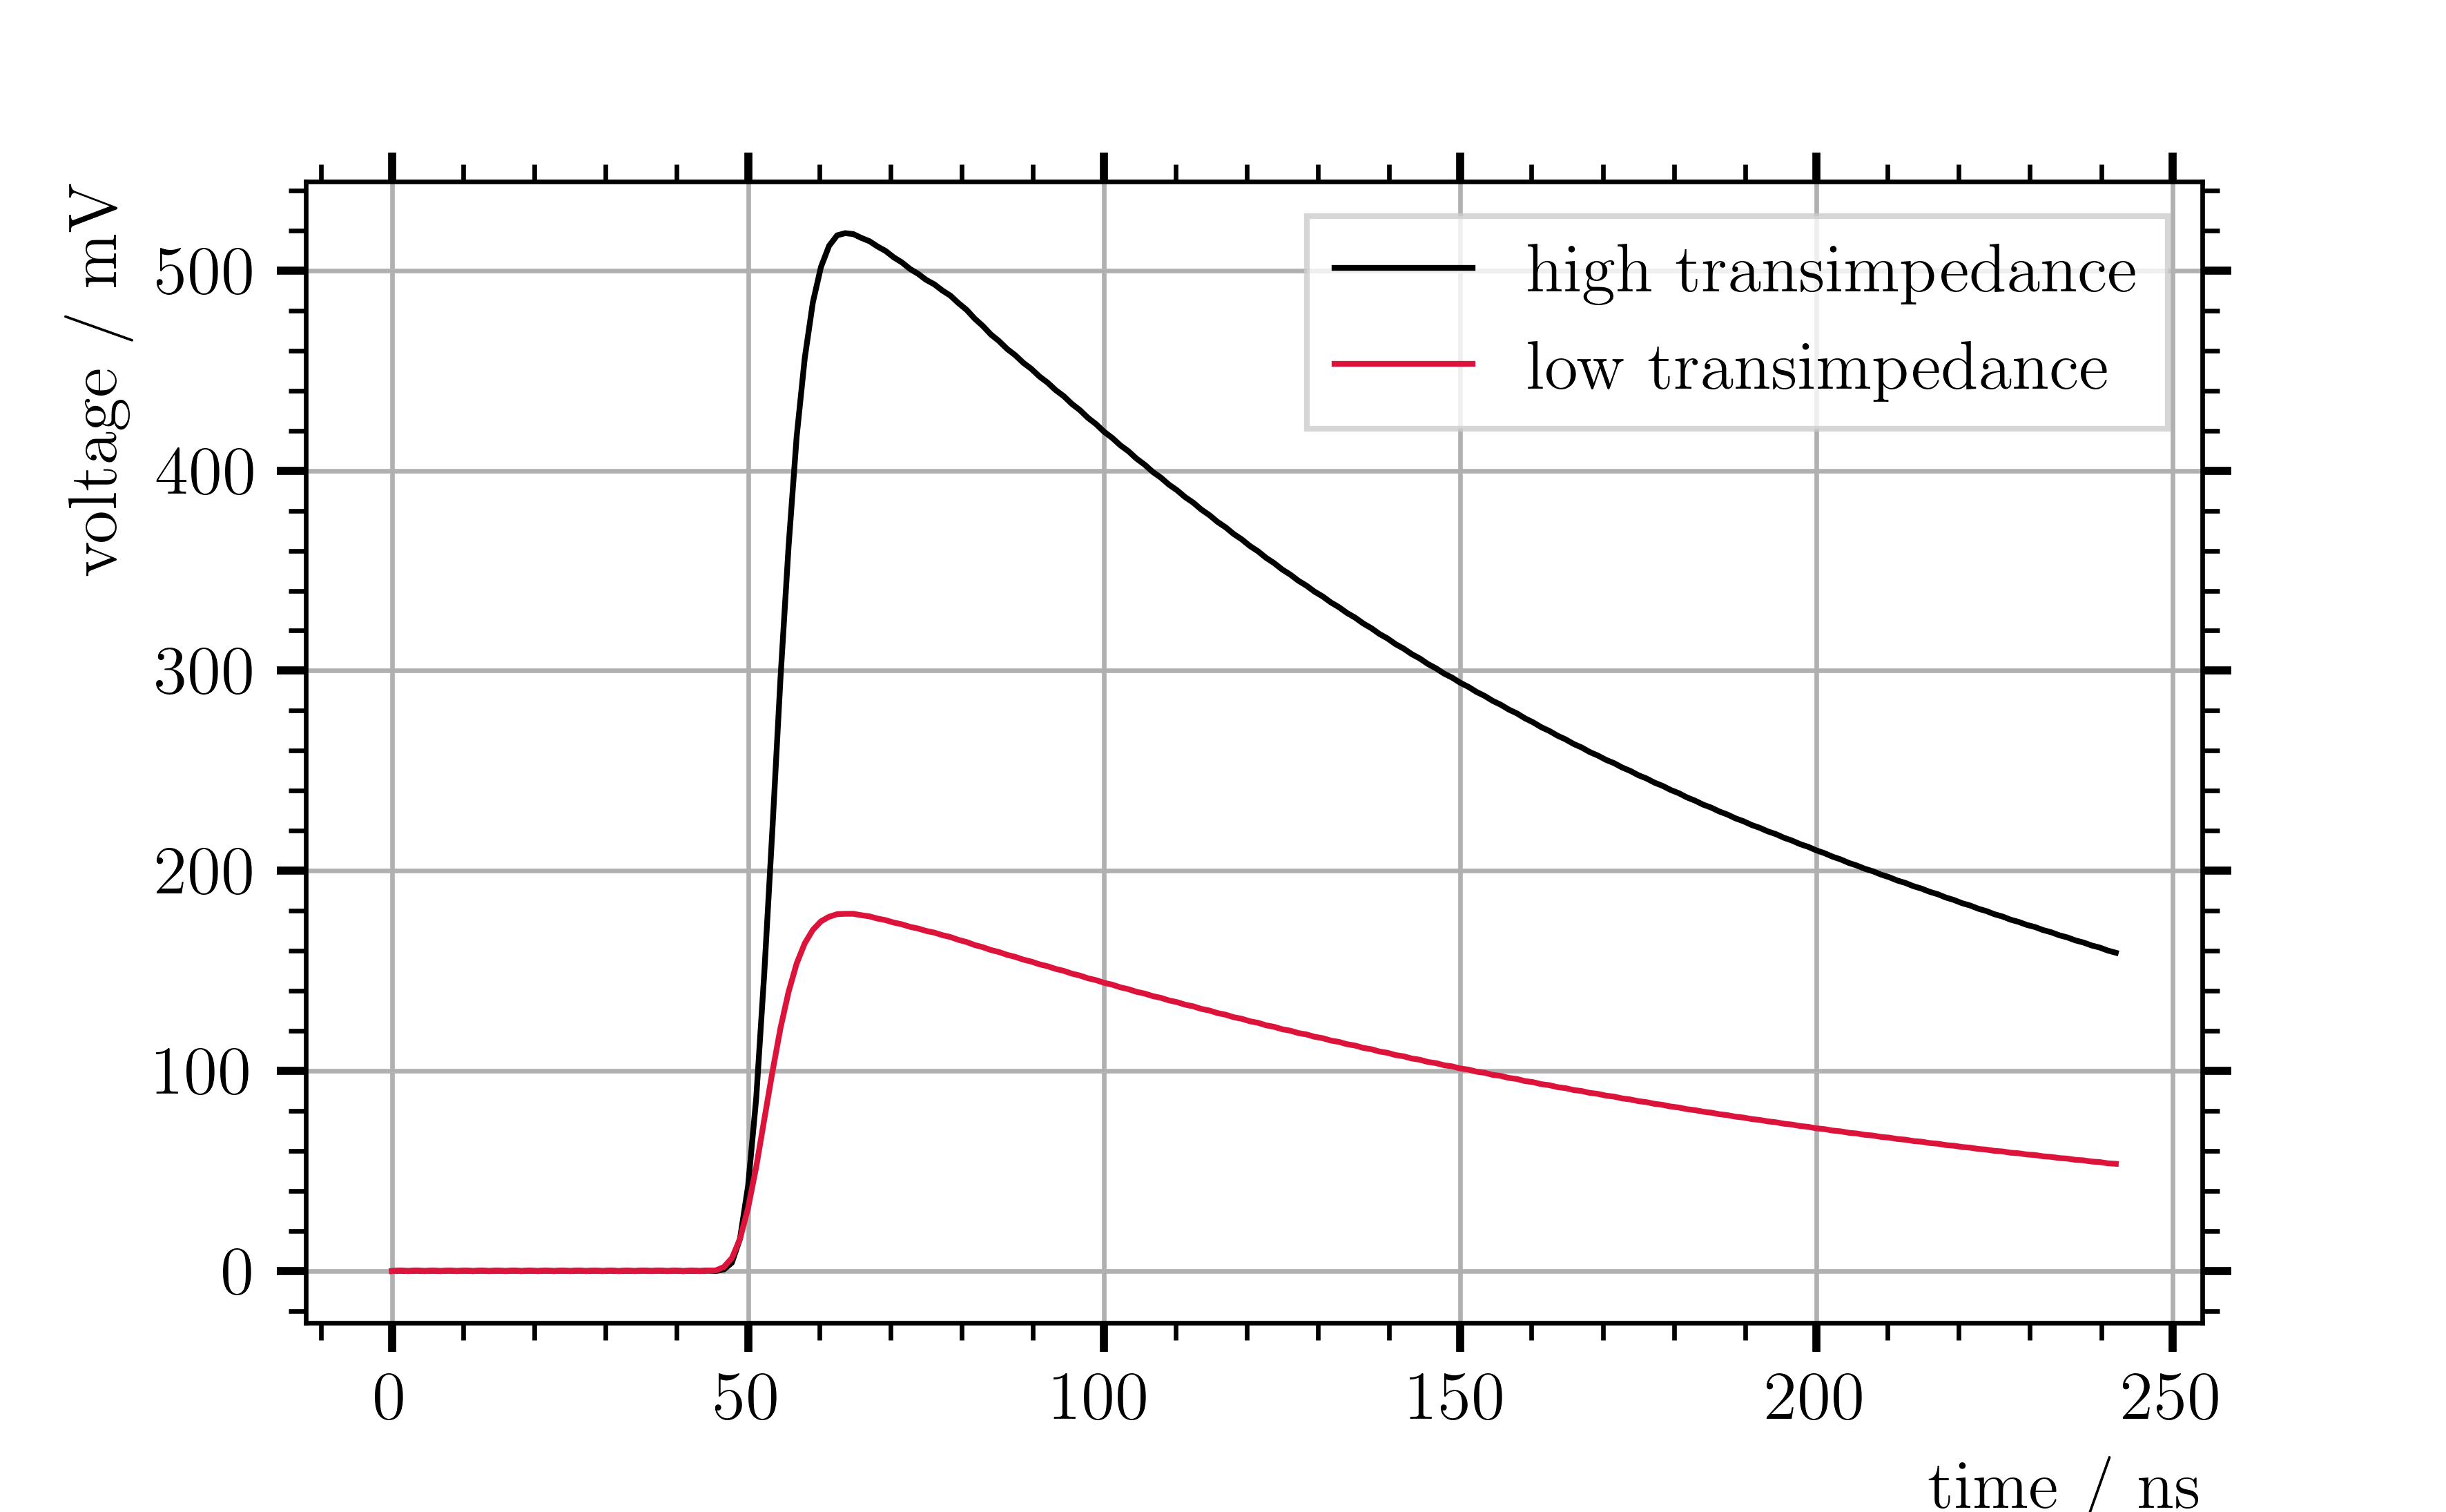
\includegraphics[width=1.\textwidth]{pictures/low_imp_mean_wf}
	\caption[Waveforms measured with low and high transimpedance]{The mean waveforms of two measurements with around \num{80000} waveforms each. The black waveform correspondes to a measurement done with high transimpedance and the red waveform correspondes to a measurement with low transimpedance.}
	\label{fig:low_imp_wf}
\end{figure}

\section{Dark Count Measurements}
Due to their indistiguishability from signals caused by photons, the measurement of dark counts can be an easy way to calibrate the readout.
To test if this is possible with the \ac{emusic} as amplifier, two dark count measurements were performed.
For the first measurement, to maximize the amplitude, the pole-zero calibration was disabled and the high transimpedance was used.
The second dark count measurement was done with enabled pole-zero calibration, low attenuation and high transimpedance.
For the resistor and capacitor of the pole-zero cancellation the settings 3 and 31 were chosen, respectively.
Since the amplitude of dark counts is in the lower \si{\milli\volt} range and therefore not much higher than the electronic noise, a measurement of the noise with a high voltage of \SI{20}{\volt} was performed for comparison.
To maximize the amplitude resolution, the oscilloscope was used instead of a \ac{gandalf} module.
In \autoref{fig:dc_hist} the histograms with the integrals of a \SI{136}{\nano\second} time window around the trigger point is shown. 
The comparisson of the dark count measurements with the noise measurement shows, that dark counts were measured.
But it no single photoelectron peaks can be distinguished with the measurement with pole-zero cancellation.
Hence, the calibration using dark count measurements is not possible in that case.
\begin{figure}
	\centering
	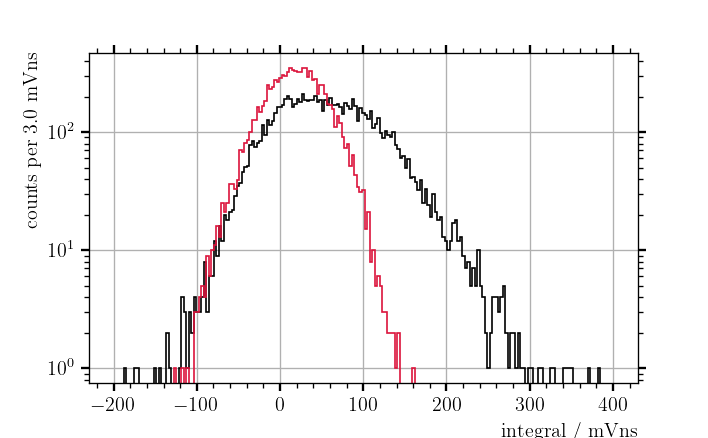
\includegraphics[width=1.\textwidth]{pictures/dc_hist_pz}
	\caption[Histogram of the dark count measurements with pole-zero cancellation.]{The histogram of the dark count measurements with pole-zero cancellation, and the electric noise measurement. No single photoelectron peaks can be distinguished in the dark count measurement histograms. Therefore dark count measurements cannot be used for calibration.} 
	\label{fig:dc_hist}
\end{figure}
The histogram with the dark count measurement result without pole-zero cancellation is shown in \autoref{fig:dc_hist_no_pz}
Also here no single photoelectron peaks can be distinguished.
Hence also without the pole-zero cancellation no calibration is possible.
\begin{figure}
	\centering
	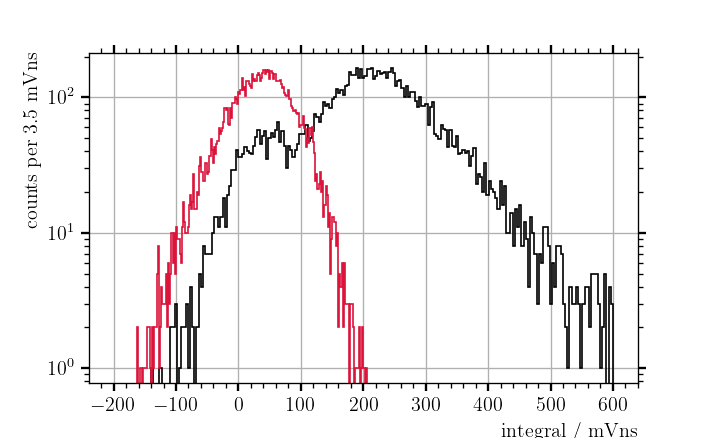
\includegraphics[width=1.\textwidth]{pictures/dc_hist_no_pz}
	\caption[Histogram of the dark count measurements without pole-zero cancellation.]{The histogram of the dark count measurements without pole-zero cancellation, and the electric noise measurement. No single photoelectron peaks can be distinguished in the dark count measurement histograms. Therefore dark count measurements cannot be used for calibration.} 
	\label{fig:dc_hist_no_pz}
\end{figure}










